\section{Controller Design}\label{sec:design}
The controller is a proportional gain $K_p$ acting on the error between the setpoint and the
measured position, both in volts, with the hover bias added afterwards. This section turns each
specification into a bound on $K_p$, takes the intersection, and then builds the result from
op-amps.

\subsection{Specifications as bounds on the gain}
\paragraph{Overshoot below 30 percent.} For a second-order system,
$OS = \exp\!\left(-\pi\zeta/\sqrt{1-\zeta^2}\right)$, so an overshoot of $0.30$ requires
\begin{equation}
    \zeta \geq \frac{-\ln 0.30}{\sqrt{\pi^2 + \ln^2 0.30}} = 0.358 .
\end{equation}
Substituting $\zeta$ from Equation~\eqref{eqn:wn_zeta} and inverting gives the ceiling
\begin{equation}\label{eqn:kp_os}
    K_p \leq \frac{1}{4\zeta_{\min}^2\,T k A} = \frac{1.951}{T k A} .
\end{equation}

\paragraph{Robustness to 10 percent in the aerodynamic constant.} A drag error does not move $T$
alone. Both $A = a/b$ and $T = 1/b$ are inversely proportional to $b$, so a single error in $b$
scales them together: the product $kAT$ in Equation~\eqref{eqn:kp_os} varies as the \emph{square}
of the error and $\zeta$ as its reciprocal, not its square root. A drag constant $10$ percent low
therefore raises $kAT$ by $21$ percent rather than $10$, and the ceiling is re-evaluated there.
Treating $T$ as the only affected parameter understates the worst corner, by $0.9$ percentage
points of overshoot in this design.

\paragraph{Robustness to 10 percent component tolerance.} A gain stage built from $10$ percent
parts may land $10$ percent above its design value, so the nominal is chosen such that the high
end of the tolerance band still satisfies the previous bound, giving $1.596/(TkA)$.

\paragraph{Tracking within 8 percent.} Equation~\eqref{eqn:fvt_error} showed the steady-state
error to a step setpoint is zero, so the whole $8$ percent budget belongs to the residual
disturbance of Equation~\eqref{eqn:fvt_dist} left after the hover bias is trimmed. For a
setpoint step $X_0$ and a residual input disturbance $d_{res}$,
\begin{equation}
    \frac{d_{res}}{K_p k} \leq 0.08\,X_0
    \qquad \Rightarrow \qquad
    K_p \geq \frac{d_{res}}{0.08\,k\,X_0} ,
\end{equation}
which is a floor rather than a ceiling. The value of $d_{res}$ is measured on the bench by
running open loop at the trimmed hover point and recording the drift, not assumed.

\paragraph{Actuator limit.} Two ceilings apply and they are not the same. The supply caps the
op-amp output at $10\ \mathrm{V}$, but the kitticopter only accepts $0$ to $5\ \mathrm{V}$, so
the usable headroom above the bias is $5 - V_h$. The error is largest at the instant of the
step, which gives
\begin{equation}\label{eqn:kp_sat}
    K_p k X_0 \leq 5 - V_h .
\end{equation}
With the bias near mid range this leaves roughly $2.5\ \mathrm{V}$, a quarter of what the supply
would allow. Beyond it the controller saturates, the loop is briefly open and the measured
overshoot stops matching the linear prediction. Which of the two ceilings binds depends on the
gain: at the gains a faster plant would permit this one would bind first, but at the
$K_p$ this plant forces, shown below to be of order $10^{-3}$, the command moves only tens of
millivolts and Equation~\eqref{eqn:kp_sat} is never approached. It is reported because it has to
be checked, not because it is active here.

\subsection{Choosing the gain}
Substituting the identified model of Equation~\eqref{eqn:identified} into the bounds above gives
numbers that do not immediately agree. The overshoot bound caps the gain at
\begin{equation}
    K_p \le \frac{1}{4\zeta_{\min}^2 k A T}
         = \frac{1}{4(0.358)^2(0.95)(23.196)(9.537)}
         = 9.3 \times 10^{-3} ,
\end{equation}
because $kAT = 210$ for this plant and the damping falls as the square root of that product. The
disturbance bound floors it at $K_p \ge \Delta V/(0.08\,r\,k)$. With the hover bias trimmed only
to the $0.1\ \mathrm{V}$ that a single-turn pot gives by eye, and a $1\ \mathrm{m}$ setpoint, that
floor is $1.3$, which is more than two orders of magnitude above the ceiling. On those numbers no
proportional controller exists.

Two things resolve it. The specification is a \emph{percentage} of the setpoint and the brief
fixes no setpoint, so a larger demonstration setpoint relaxes the floor proportionally. And the
residual is proportional to the bias trim error, so trimming against a meter rather than by eye
lowers the floor directly. Taking a $7\ \mathrm{m}$ setpoint and a $2\ \mathrm{mV}$ trim,
\begin{equation}\label{eqn:kp_floor}
    K_p \ge \frac{\Delta V}{0.08\,r\,k} = \frac{0.002}{0.08(7)(0.95)} = 3.8 \times 10^{-3} ,
\end{equation}
and a window opens. Across every corner of the tolerance budget it is $K_p = 0.005$ to $0.006$,
and the chosen value is

\begin{equation}
    K_p = 0.005 , \qquad
    \omega_n = \sqrt{\frac{K_p k A}{T}} = 0.107\ \mathrm{rad\,s^{-1}} , \qquad
    \zeta = \frac{1}{2\sqrt{K_p k A T}} = 0.488 ,
\end{equation}
predicting $17.3$ percent overshoot and a $2$ percent settling time of $76\ \mathrm{s}$.

The setpoint is then capped from above by the sensor, which saturates at $10\ \mathrm{V}$, or
$10.5\ \mathrm{m}$. A setpoint that overshoots past that opens the feedback path at the moment the
loop is being judged. At the worst corner the overshoot is $26.7$ percent, so $7\ \mathrm{m}$
peaks at $8.9\ \mathrm{m}$ and stays clear, while the $10\ \mathrm{m}$ that would widen the gain
window peaks at $12.5$ and clips. The setpoint is set by the sensor range, not the gain window.

Table~\ref{tab:corners} in Appendix~\ref{sec:appendix} walks all nine corners, formed as described
above with $A$ and $T$ moving together. The worst case is $26.7$ percent overshoot and $4.6$
percent offset, both inside specification. A Monte Carlo of $20\,000$ builds drawn uniformly from
the same tolerance boxes passes all three specifications in $100$ percent of cases, so the corner
result is not a knife edge.

One property of this plant is worth stating because it limits what proportional control can do
here. The decay envelope is set by $\zeta\omega_n = 1/(2T)$, which does not contain $K_p$, so
the settling time cannot be improved by raising the gain. Raising $K_p$ raises $\omega_n$ and
makes the response ring more without making the envelope decay faster. That is the limitation
compensation exists to fix.

\subsection{Simulation}
Figure~\ref{fig:closed_loop_step} shows the nominal closed-loop step and the same response
across the component tolerance. The design is checked in simulation before it is built, with the plant swept $\pm 10$ percent in
$b$ and the gain swept $\pm 10$ percent to cover both robustness specifications, and with the
$0$ to $5\ \mathrm{V}$ input saturation included, since a linear simulation would hide exactly
the effect that Equation~\eqref{eqn:kp_sat} warns about.

\begin{figure}[htbp]
    \centering
    \begin{minipage}{0.49\textwidth}\centering
        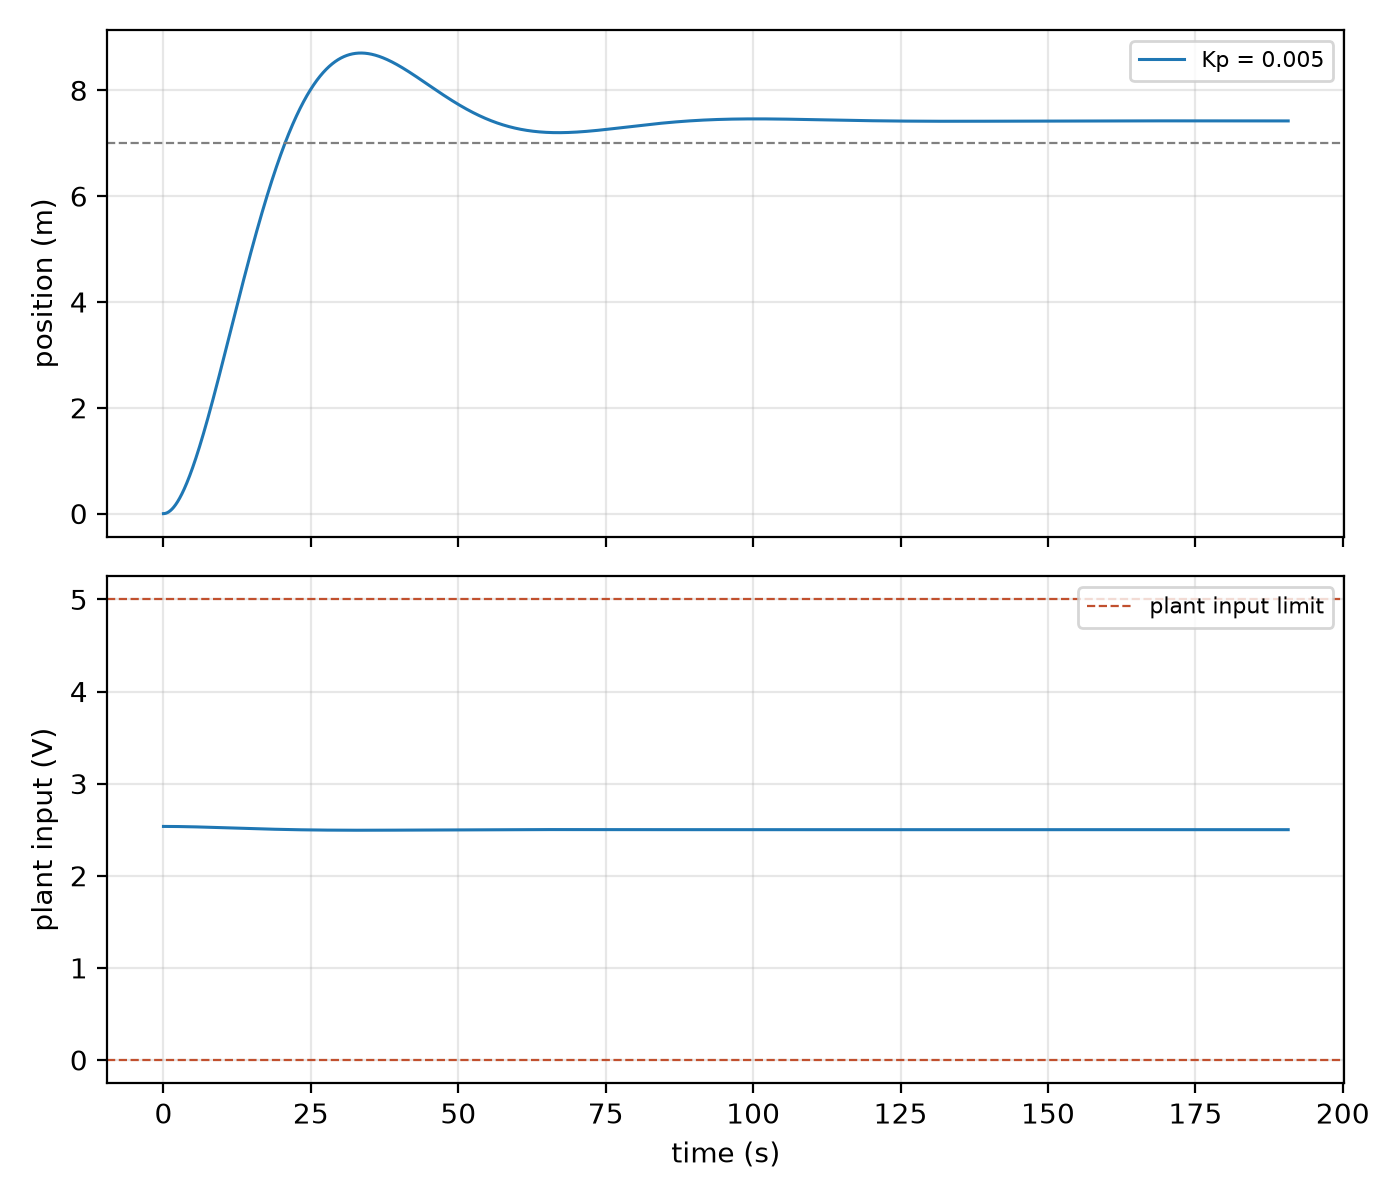
\includegraphics[width=\textwidth]{figures/closed_loop_step.png}
    \end{minipage}\hfill
    \begin{minipage}{0.49\textwidth}\centering
        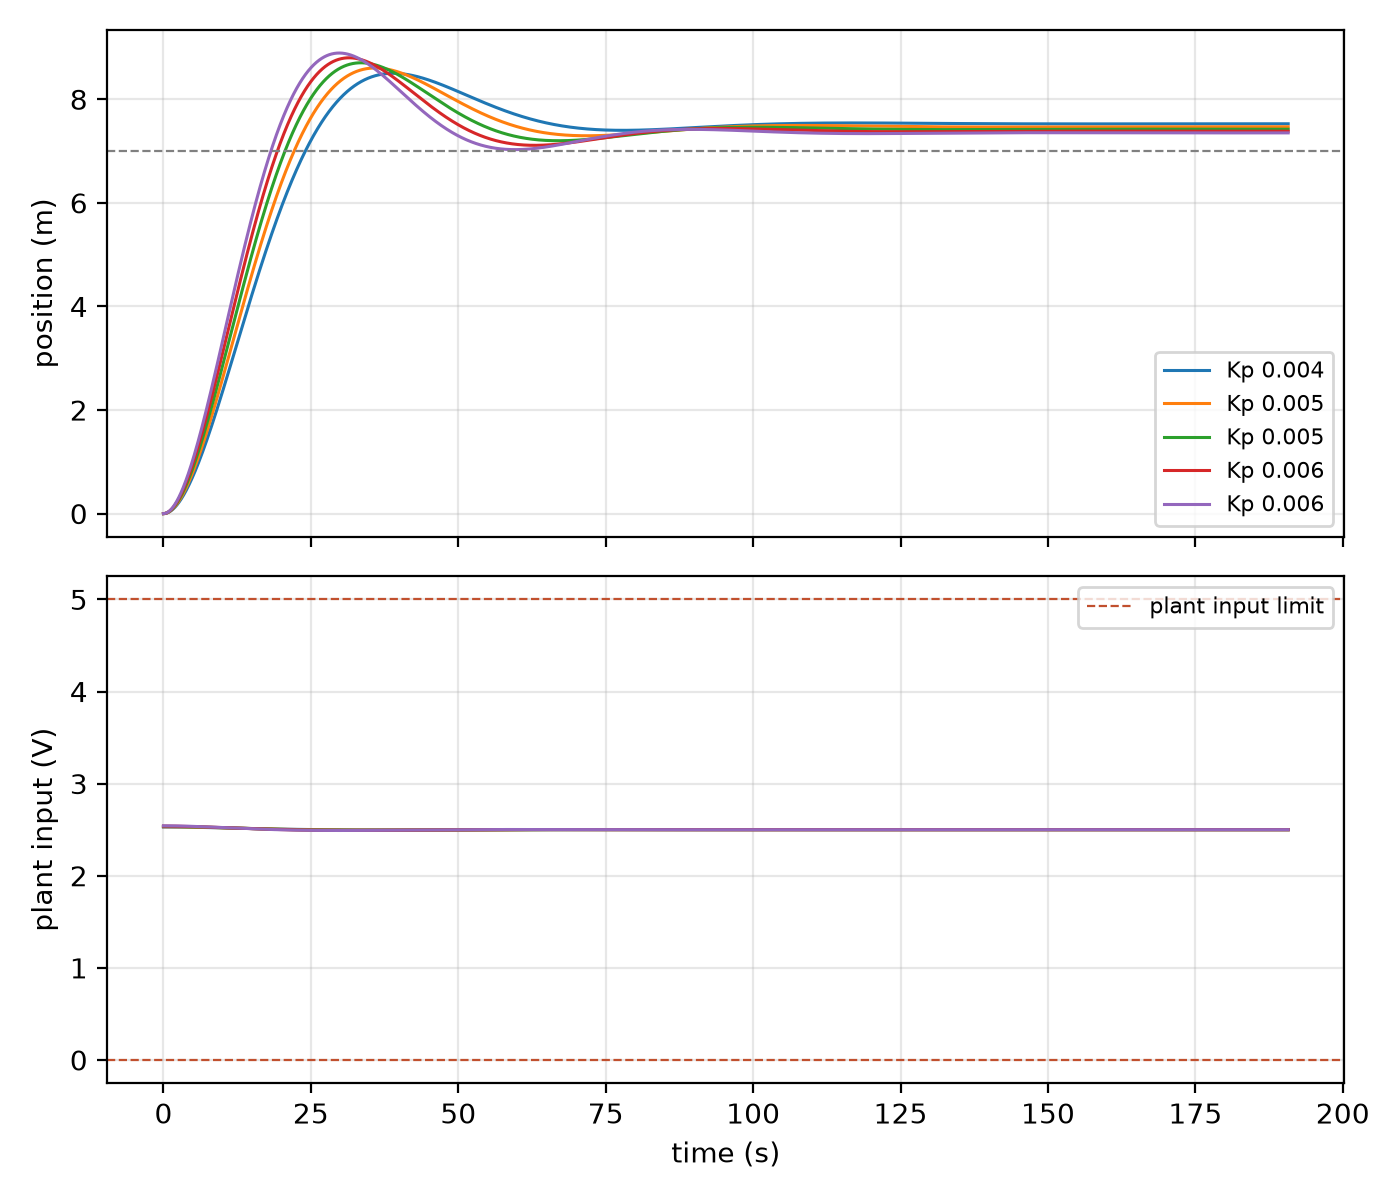
\includegraphics[width=\textwidth]{figures/robustness_kp.png}
    \end{minipage}
    \caption{Left: simulated closed-loop step to $7\ \mathrm{m}$ at $K_p = 0.005$ with a
    $2\ \mathrm{mV}$ bias error. Height settles at $7.42\ \mathrm{m}$, a $6.0$ percent offset,
    with $17.3$ percent overshoot, and the command stays between $2.49$ and $2.54\ \mathrm{V}$ so
    the saturation block never acts. Right: the same response with the gain swept $\pm 10$
    percent. Overshoot runs $13.0$ to $21.0$ percent and the offset $7.5$ to $5.0$, both inside
    specification across the whole component tolerance, and moving in opposite directions, which
    is the tradeoff that set the window.}
    \label{fig:closed_loop_step}
\end{figure}

Three independent routes agree on the overshoot: $17.29$ percent from
Equation~\eqref{eqn:wn_zeta} by hand, $17.28$ from the Python integration of
Figure~\ref{fig:closed_loop_step}, and $17.02$ from a \textsc{Simulink} model of the same loop
built separately. The agreement confirms the second-order formulas are being applied to the right
transfer function rather than matching by accident.



Figure~\ref{fig:robustness_bias} in Appendix~\ref{sec:appendix} is the practical conclusion of the
design: the steady-state error is set almost entirely by the bias trim, not the gain, so bench time
belongs at the level shifter rather than on hunting a better $K_p$.

\subsection{Circuit implementation}
The controller is assembled from three op-amp stages, following Appendix A1 of the lab brief.

\begin{enumerate}
    \item A \textbf{differential amplifier} forms the error, with all four resistors equal so
    that $V_{out} = V_{+} - V_{-}$. Its ability to reject the common-mode part of the two inputs
    depends on how well those four resistors match, which $10$ percent parts do not guarantee,
    so they are measured and paired by hand.
    \item A \textbf{non-inverting gain stage} applies $K_p = 1 + R_1/R_2$. This form cannot
    produce a gain below unity, so a design calling for $K_p < 1$ needs an inverting stage
    followed by a second inversion instead.
    \item A \textbf{summing stage} adds the hover bias $V_h$, taken from a divider off the
    $15\ \mathrm{V}$ rail, so that the command presented to the ADC sits inside the $0$ to
    $5\ \mathrm{V}$ window.
\end{enumerate}

The gain is set with a trimpot rather than a fixed pair, which turns the $10$ percent component
tolerance from a constraint that has to be absorbed in the design into something trimmed out on
the bench. The tolerance analysis above is still reported, since the specification asks for the
margin to be shown.

Because $K_p = 0.005$ is far below unity, stage 2 is built as an inverting attenuator rather than
the non-inverting form, and stage 3 is wired as a second differential amplifier rather than a
summer so that it restores the sign while adding the bias. With $V_{bias}$ on the non-inverting
side and $-K_pV_e$ on the inverting side, all four resistors equal,
\begin{equation}
    V_{cmd} = V_{bias} - \left(-K_p V_e\right) = V_{bias} + K_p V_e ,
\end{equation}
which is the command the plant needs. Figure~\ref{fig:schematic} is the resulting circuit and
Table~\ref{tab:bom} its component list.

\begin{figure}[htbp]
    \centering
    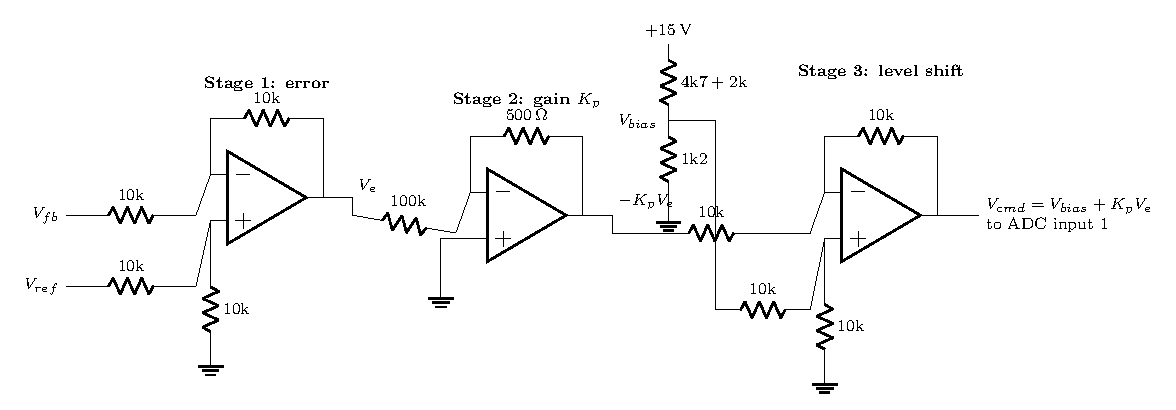
\includegraphics[width=0.92\textwidth]{figures/schematic.pdf}
    \caption{The three-stage proportional controller. Stage 1 forms the position error, stage 2
    attenuates it by $K_p$ and inverts, stage 3 restores the sign and adds the hover bias. All
    three stages are UA741 devices on $\pm 15\ \mathrm{V}$ rails.}
    \label{fig:schematic}
\end{figure}

\begin{table}[htbp]
\centering
\caption{Component values. The two trimmers are the only adjustments made on the bench.}
\label{tab:bom}
\begin{tabular}{llll}
\toprule
Stage & Part & Value & Purpose \\
\midrule
1 & $R_1$ to $R_4$ & $10\ \mathrm{k\Omega}$ & unity-gain difference, $V_e = V_{ref} - V_{fb}$ \\
2 & $R_{in}$ & $100\ \mathrm{k\Omega}$ & sets $K_p = R_f/R_{in}$ \\
2 & $R_f$ & $1\ \mathrm{k\Omega}$ trimmer at $500\ \Omega$ & $K_p = 0.005$, trims the window \\
3 & $R_9$ to $R_{12}$ & $10\ \mathrm{k\Omega}$ & unity-gain difference, restores sign \\
3 & upper divider & $4\mathrm{k}7 + 2\ \mathrm{k\Omega}$ trimmer & sets $V_{bias}$ \\
3 & lower divider & $1\mathrm{k}2$ & sets $V_{bias}$ \\
\bottomrule
\end{tabular}
\end{table}

\paragraph{Loading of the bias divider.} The divider cannot be designed on its own, because the
$10\ \mathrm{k\Omega}$ input resistor of stage 3 loads it. A divider giving exactly
$2.50\ \mathrm{V}$ unloaded delivers only $2.35\ \mathrm{V}$ once connected, and
Figure~\ref{fig:robustness_bias} shows that $0.15\ \mathrm{V}$ error would be a $450$ percent
steady-state offset. Solving the loaded expression, derived in Appendix~\ref{sec:appendix}, gives
$5.65\ \mathrm{k\Omega}$ for the upper leg, which is why it is a $4\mathrm{k}7$ in series with a
$2\ \mathrm{k\Omega}$ trimmer. An \textsc{ngspice} simulation of the three stages with a
behavioural UA741 confirms both this level, at $2.504\ \mathrm{V}$, and the gain, at
$+0.005\ \mathrm{V/V}$, the positive sign showing the two inversions cancel as intended. That
check is also in Appendix~\ref{sec:appendix}.

\paragraph{Trimming procedure.} The two trimmers are set in a fixed order, and the second is set
with the loop closed. The gain trimmer is set first, open loop, by measuring the ratio of stage 2
output to stage 1 output. The bias trimmer is then set with the kitticopter connected and the
setpoint equal to the current height, adjusting until the kitticopter holds station. Trimming this
way rather than metering $2.500\ \mathrm{V}$ at the output absorbs the offset voltages of all
three UA741 devices, which are specified at $1\ \mathrm{mV}$ typical and $5\ \mathrm{mV}$ maximum
each and would otherwise consume the entire $2\ \mathrm{mV}$ budget that
Equation~\eqref{eqn:kp_floor} depends on.

% Awaiting the build: a photo of the finished Veroboard.
